\subsection{拓扑群}

在本章前四节中，群的合成法则一般写成乘法形式，并用 e 表示单位元；把结果改写成加法记号（我们提醒读者，加法记号专用于交换群）通常留给读者完成。

定义 1. 拓扑群是带有一个群结构和一个拓扑并且满足下列两条公理的集合 G：

\((\mathrm{GT}_{\mathbf{I}})\)。映射 \((x, y) \to xy\)（\(\mathbf{G} \times \mathbf{G}\) 到 \(\mathbf{G}\) 中的）是连续的。

\((\mathbf{G}\mathbf{T}_{\mathbf{II}})\)。映射 \(x \to x^{-1}\)（\(\mathbf{G}\) 到 \(\mathbf{G}\) 中的，即群 \(\mathbf{G}\) 的对称映射）是连续的。

集合 G 上的一个群结构与一个拓扑称为相容的，如果它们满足 \((\mathrm{GT}_{\mathbf{I}})\) 与 \((\mathrm{GT}_{\mathbf{II}})\)。

例。1) 群 G 上的离散拓扑与该群结构相容。拓扑为离散的拓扑群称为离散群。

又如，G 上的最粗拓扑（第一章 § 2 第 2 目）与 G 的群结构相容。

* 2) 在第四章我们将看到，有理直线 Q（相应地，实直线 R）的拓扑与 Q（相应地，R）的加法群结构相容。*

\begin{enumerate}
\def\labelenumi{\arabic{enumi})}
\setcounter{enumi}{2}
\tightlist
\item
  若 G 是拓扑群，则它的拓扑与 G 的反群 \(G^{0}\) 的结构相容；赋有这个拓扑的 \(G^{0}\) 称为 G 的反拓扑群。
\end{enumerate}

公理 \((\mathrm{GT}_{\mathrm{I}})\) 与 \((\mathrm{GT}_{\mathrm{II}})\) 等价于下列公理：

\((\mathbf{GT}^{\prime})\)。映射 \((x,y)\to xy^{-1}\)（\(\mathbf{G}\times \mathbf{G}\) 到 \(\mathbf{G}\) 中的）是连续的。

显然 \((\mathrm{GT}_{\mathbf{I}})\) 与 \((\mathrm{GT}_{\mathbf{II}})\) 合起来蕴涵 \((\mathrm{GT}^{\prime})\)。反之，\((\mathrm{GT}^{\prime})\) 蕴涵 \((\mathrm{GT}_{\mathbf{II}})\)，因为这时 \(x \to ex^{-1} = x^{-1}\) 是连续的；而 \((\mathrm{GT}^{\prime})\) 与 \((\mathrm{GT}_{\mathbf{II}})\) 合起来蕴涵 \((\mathrm{GT}_{\mathbf{I}})\)，因为这时 \((x, y) \to x(y^{-1})^{-1} = xy\) 是连续的。

若 \(a\) 是 \(G\) 的任意元素，则左平移 \(x \to ax\)（相应地，右平移 \(x \to xa\)）由 \((GT_{I})\) 是连续的，因而是 \(G\) 到 \(G\) 上的一个同胚。诸映射 \(x \to axb\)（当 \(a\) 与 \(b\) 取遍 \(G\) 时）组成 \(G\) 的一个同胚群；诸映射 \(x \to axa^{-1}\)（相应地 \(x \to ax\)、\(x \to xa\)），其中 \(a\) 取遍 \(G\)，组成这个同胚群的一个子群。又，由于对称映射 \(x \to x^{-1}\) 是 \(G\) 的一个对合置换，公理 \((GT_{II})\) 表明这个映射是 \(G\) 到 \(G\) 上的一个同胚。

若 A 是 G 的开（相应地，闭）子集，x 是 G 的任意一点，则集 x.A、A.x 与 \(A^{-1}\) (*) 都是开（相应地，闭）的，因为它们都是 A 在上述某个同胚下的像。若 A 是开集而 B 是 G 的任意子集，则 AB 与 BA 都是开集，因为它们都是开集的并{[}公理 \((\mathrm{O}_{\mathrm{I}})\){]}。若 V 是 G 中 e 的邻域，则 VA 与 AV 都是 A 的邻域；因为若 W 是包含在 V 中的 e 的开邻域，则 WA 与 AW 都是开集并且包含 A。

\pandocbounded{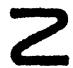
\includegraphics[keepaspectratio]{images/part002_a77d6c20.jpg}}

另一方面，当 A 是闭集时，即使 B 也是闭集，AB 也未必是闭集（参看 § 4 第 1 目命题 1 的推论 1）。

* 例如，在实直线 \(\mathbf{R}\) 的加法群中，有理整数组成的子群 \(\mathbf{Z}\) 是闭的，子群 \(\theta\mathbf{Z}\)（由全体整数倍 \(n\theta\)（\(\theta\) 为一无理数）组成）也是闭的；但子群 \(\mathbf{Z} + \theta\mathbf{Z}\)（\(\mathbf{R}\) 的），即实数 \(m + n\theta\)（其中 \(m\) 与 \(n\) 取遍一切整数值）组成的集，在 \(\mathbf{R}\) 中不是闭的，这一点我们将在第五章 § 1 中看到。

又，设 A 是 \(\mathbf{R} \times \mathbf{R}\) 的加法群中由全体点对 \((x, y)\)（满足 \(x \geqslant 0\) 与 \(0 \leqslant y \leqslant 1 - \frac{1}{x + 1}\) 的）组成的子集；并设 B 是当 x 取遍 R 时全体点对 \((x,0)\) 组成的集。A 与 B 都是闭的，但 \(A + B\) 是由全体点对 \((x,y)\)（满足 \(0 \leqslant y < 1\) 的）组成的集，它在 \(R \times R\) 中不是闭的。

设 X 是拓扑空间，f 与 g 是 X 到拓扑群 G 中的两个映射。若 f 与 g 在 X 的一点 \(x_{0}\) 处连续，则由第一章 § 2 第 1 目定理 2，\(\overline{f}^{1}\) 与 \(fg\) (*) 也连续。特别地，X 到 G 中的连续映射组成 X 到 G 的一切映射所成的群 \(\mathbf{G}^{\mathbf{x}}\) 的一个子群。

又，设 \(f\) 与 \(g\) 是集合 \(\mathbf{X}\)（由滤子 \(\mathfrak{F}\) 装备的）到 Hausdorff 拓扑群 \(\mathbf{G}\) 中的两个映射。若 \(\lim_{\mathfrak{F}} f\) 与 \(\lim_{\mathfrak{F}} g\) 存在，则 \(\lim_{\mathfrak{F}} \overline{f}^1\) 与 \(\lim_{\mathfrak{F}} fg\) 也存在，并且我们有（第一章 § 7 第 4 目命题 9 的推论 1）

\[
\lim _ {\mathfrak {F}} \overline {{f}} ^ {- 1} = (\lim _ {\mathfrak {F}} f) ^ {- 1},\tag{1}
\]

\[
\lim _ {\mathfrak {F}} f g = (\lim _ {\mathfrak {F}} f) (\lim _ {\mathfrak {F}} g).\tag{2}
\]

当 G 是写成加法形式的交换群时，公理 (GT') 表明 \((x, y) \to x - y\) 是连续映射。若 f 与 g 是拓扑空间 X 到 G 中的映射，并且在一点 \(x_{0}\) 处连续，则 f - g 在该点连续。公式 (1) 与 (2) 可以类似地改写。
% semantic-fragments: legacy-input-seam
\relax{}
